% example tikz figure

\documentclass{standalone}
\usepackage{amsmath}
\usepackage{tikz}
\usetikzlibrary{arrows,shapes,positioning,shadows,trees}

\begin{document}
\begin{tikzpicture}
    \node (a) at (0,0) {
        \begin{tikzpicture}
            \filldraw[fill=gray!20,draw=white] (-2,1) rectangle (2,-1);
            \draw[-] (-2,0) -- (2,0);
            \draw[-] (0,-2) -- (0,2);
            \draw[-] (-2,1) -- (2,1);
            \draw[-] (-2,-1) -- (2,-1);
            \node[anchor=south west] at (0,1) {$i\theta$};
        \end{tikzpicture}
    };

    \node (b) at (8,0) {
        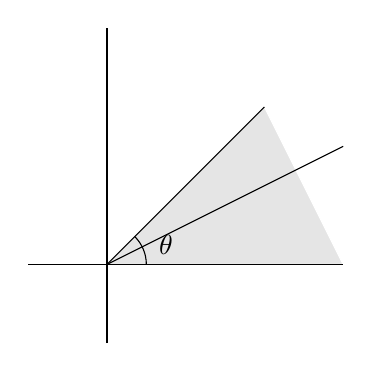
\begin{tikzpicture}
            \filldraw[fill=gray!20,draw=white] (0,0) -- (2,2) -- (3,0) -- (0,0);
            \draw[-] (-1,0) -- (3,0);
            \draw[-] (0,-1) -- (0,3);
            \draw[-] (0,0) -- (2,2);
            \draw[-] (0,0) -- (3,1.5);
            \draw (0.5,0) arc (0:45:0.5);
            \node at (0.75,0.25) {$\theta$};
        \end{tikzpicture}
    };

    \node (c) at (16,0) {
        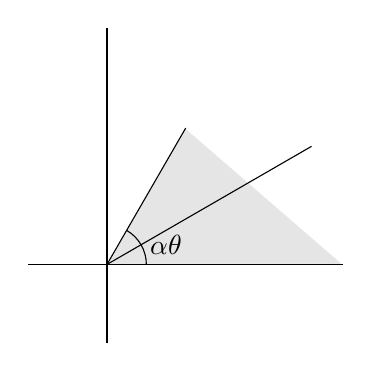
\begin{tikzpicture}
            \filldraw[fill=gray!20,draw=white] (0,0) -- (1,1.732) -- (3,0) -- (0,0);
            \draw[-] (-1,0) -- (3,0);
            \draw[-] (0,-1) -- (0,3);
            \draw[-] (0,0) -- (1,1.732);
            \draw[-] (0,0) -- (1.732 * 1.5,1 * 1.5);
            \draw (0.5,0) arc (0:60:0.5);
            \node at (0.75,0.25) {$\alpha\theta$};
        \end{tikzpicture}
    };

    \draw[->] (a) -- (b) node[midway,above] {$e^z$};
    \draw[->] (b) -- (a) node[midway,below] {$\log z$};
    \draw[->] (b) -- (c) node[midway,above] {$z^{\alpha} (\alpha > 0)$};
\end{tikzpicture}
\end{document}